\documentclass[a4paper,11pt]{article}

\usepackage{amsmath}
\usepackage[pdftex]{graphicx}

\usepackage[english,greek]{babel}

\usepackage{lmodern}

\usepackage{listings}

\lstset{
  basicstyle=\ttfamily,
  columns=fullflexible,
  frame=single,
  breaklines=true
}

% Αφαίρεσε (Εισήγαγε) την παρακάτω γραμμή σε σχόλιο αν ο επεξεργαστής κειμένου (δεν) χρησιμοποιεί κωδικοποίηση Unicode για Ελληνικά
\usepackage[utf8x]{inputenc}

% Αφαίρεσε (Εισήγαγε) την παρακάτω γραμμή σε σχόλιο αν ο επεξεργαστής κειμένου (δεν) χρησιμοποιεί κωδικοποίηση iso-8859-7 για Ελληνικά
%\usepackage[iso-8859-7]{inputenc}

%Δημιουργία συντομεύσεων για αλλαγή γραφής σε Ελληνικά/Αγγλικά
\newcommand{\lt}{\latintext}
\newcommand{\gt}{\greektext}

\title{1η Υποχρεωτική Εργασία \\ Στο Μάθημα της Αριθμητικής Ανάλυσης: \\ Άσκηση 2}
\author{Όνοματεπώνυμο: Μπαρακλιλής Ιωάννης  \\  ΑΕΜ: 3685}
\date{17 Δεκεμβρίου 2020}

\begin{document}

\maketitle

\section{Ζητούμενο (α): Τροποποιημένη μέθοδος {\lt Newton-Raphson}}
Ζητείται η υλοποίηση μίας τροποποιημένης μεθόδου {\lt Newton-Raphson} με \lt \[x_{n+1} = x_n - \dfrac{f(x_n)}{f'(x_n)} - \dfrac{1}{2}\dfrac{f(x_n)^2f''(x_n)}{f'(x_n)^3} \].

\gt

Η μέθοδος αυτή υλοποιείται προγραμματιστικά στην γλώσσα {\lt python} (3.7) στο αρχείο {\lt a\textunderscore Modified\textunderscore Newton\textunderscore Raphson.py} το οποίο φαίνεται παρακάτω:

\lt
\lstinputlisting[language=Python]{a_Modified_Newton_Raphson.py}
\gt

Στον παραπάνω κώδικα:\\
Ορίζω την συνάρτηση {\lt modified\textunderscore newton\textunderscore raphson} η οποία δέχεται την συνάρτηση, την πρώτη και δεύτερη παράγωγο της συνάρτησης, το αρχικό σημείο της ακολουθίας και τα ζητούμενα ψηφία ακρίβειας:\par
Αρχικά, ορίζω ψευδώνυμα για την συνάρτηση και την πρώτη και δεύτερη παράγωγο της (με ονόματα {\lt f}, {\lt f\textunderscore d} και {\lt f\textunderscore dd} αντίστοιχα).
Επίσης, ορίζω και αρχικοποιώ την μεταβλητή {\lt iteration\textunderscore counter}, σε 0,  που <<μετράει>> τις επαναλήψεις της μεθόδου και την μεταβλητή {\lt x}, στο αρχικό σημείο της ακολουθίας (που δίνεται ως όρισμα), που αποθηκεύει την τρέχουσα εκτίμηση της ρίζας.

Στην συνέχεια, αρχίζει ατέρμονος βρόχος (που θα τερματισει αργότερα όταν <<πετύχω>> την επιθυμιτή ακρίβεια) όπου γίνονται οι ενέργειες:\\
Πρώτα, ελέγχω αν η τρέχουσα εκτίμηση αποτελεί ρίζα της συνάρτησης, επειδή αν ισχύει αυτό δεν χρειάζεται να συνεχίσω την αναζήτηση γιατί βρέθηκε η ζητούμενη ρίζα. Άν είναι τερματίζω την εκτέλεση της συνάρτησης και επιστρέφω την εκτίμηση της ρίζας και τον αριθμό των επαναλήψεων που χρειάστηκαν για να βρεθεί.\\
Στην συνέχεια (η τρέχουσα εκτίμιση δεν αποτελεί ρίζα): ενημερώνω την μεταβλητή που αποθηκεύει τον αριθμό των επαναλήψεων, υπολογίζω το επόμενο στοιχείο ακολουθίας που αποτελεί την επόμενη εκτίμηση της ρίζας ($x_{n+1} = x_n - \dfrac{f(x_n)}{f'(x_n)} - \dfrac{1}{2}\dfrac{f(x_n)^2f''(x_n)}{f'(x_n)^3}$) και το αποθηκεύω στην (νέα) μεταβλητή {\lt x\textunderscore next}.\\
Τέλος, ελέγχω άν η διαφορά της νέας και παλιάς εκτίμησης (διαφορά μεταβλητών {\lt x} και {\lt x\textunderscore next} είναι μικρότερη του ανεκτού σφάλματος και αν είναι επιστρέφω την εκτίμηση της ρίζας και τον αριθμό των επαναλήψεων που χρειάστηκαν για να βρεθεί (τερματίζοντας την εκτέλεση της συνάρτησης).

\section{Ζητούμενο (β): Τροποποιημένη μέθοδος διχοτόμησης}
Ζητείται η υλοποίηση μίας τροποποιημένης μεθόδου διχοτόμησης όπου η εκτίμηση για την ρίζα δεν είναι το μέσο του
διαστήματος αναζήτησης σε κάθε βήμα αλλά ένα τυχαίο σημείο που επιλέγεται με την χρήση μιας
συνάρτησης παραγωγής τυχαίων αριθμών εντός του διαστήματος αναζήτησης. Η επιλογή τυχαίου σημείου εντός διαστήματος μπορεί να γίνει με την χρήση της συνάρτησης {\lt uniform}, του {\lt module random}, που επιστρέφει έναν τυχαίο πραγματικό αριθμό εντός του διαστήματος τα άκρα του οποίου που δίνονται ως παράμετροι.

Η μέθοδος αυτή υλοποιείται προγραμματιστικά στην γλώσσα {\lt python} στο αρχείο {\lt b\textunderscore Modified\textunderscore Bisection.py} το οποίο φαίνεται παρακάτω:

\lt
\lstinputlisting[language=Python]{b_Modified_Bisection.py}
\gt

Ο παραπάνω κώδικας είναι πανομοιότυπος με τον αντίστοιχο του ερωτήματος (α) της άσκησης 1, που υλοποιεί την κλασσική μέθοδο διχοτόμησης, με την διαφορά ότι η νέα εκτίμηση ρίζας υπολογίζεται ως τυχαίο σημείο εντός του διαστήματος αναζήτησης αντί του μέσου αυτού του διαστήματος.

Παρ'' όλα αυτά, είναι χρήσιμο να αναλυθεί (έκ νέου) η λειτουργία του παραπάνω κώδικα:
\\
Oρίζω την συνάρτηση {\lt modified\textunderscore bisection} η οποία δέχεται την συνάρτηση, το αριστερό άκρο του αρχικού διαστήματος, το δεξί άκρο του αρχικού διαστήματος και τα ζητούμενα ψηφία ακρίβειας:\par
Αρχικά, ορίζω ψευδώνυμα για την συνάρτηση, αρχή και τέλος διαστήματος αναζήτησης ρίζας (με ονόματα {\lt f, a, b} αντίστοιχα).
Ακόμη, ορίζω και αρχικοποιώ την μεταβλητή {\lt iteration\textunderscore counter}, σε 0,  που <<μετράει>> τις επαναλήψεις της μεθόδου.
Επίσης, ορίζω και δίνω τιμές στις μεταβλητές που αποθηκεύουν την τιμή συνάρτησης στην αρχή και τέλος διαστήματος, το τυχαίο σημείο του διαστήματος και την τιμή συνάρτησης στο τυχαίο σημείο διαστήματος (με ονόματα {\lt fa, fb, r, fr} αντίστοιχα). 


Στην συνέχεια, αρχίζει ατέρμονος βρόχος (που θα τερματισει αργότερα όταν <<πετύχω>> την επιθυμιτή ακρίβεια) όπου γίνονται οι ενέργειες:\\
Πρώτα, ελέγχω αν η τρέχουσα εκτίμηση (τυχαίο σημείο του διαστήματος) αποτελεί ρίζα της συνάρτησης, επειδή αν ισχύει αυτό δεν χρειάζεται να συνεχίσω την αναζήτηση γιατί βρέθηκε η ζητούμενη ρίζα. Άν είναι τερματίζω την εκτέλεση της συνάρτησης και επιστρέφω την εκτίμηση της ρίζας και τον αριθμό των επαναλήψεων που χρειάστηκαν για να βρεθεί.\\
Στην συνέχεια (η τρέχουσα εκτίμιση δεν αποτελεί ρίζα), υπολογίζω το νέο διάστημα αναζήτησης: Άν το γινόμενο της συνάρτησης στο αριστερό άκρο ({\lt a}) με την συνάρτηση στο τυχαίο σημείο του διαστήματος ({\lt r}) είναι αρνητικό ({\lt $fa * fr < 0$}) τότε έχω ρίζα στο διάστημα $[a, r]$ και ορίζω νέο διάστημα αναζήτησης ορίζοντας ως νέο δεξί άκρο διαστήματος το τυχαίο σημείο (θέτω {\lt b = r} και για να μην το ξαναυπολογίσω θέτω {\lt fb = fr}). Διαφορετικά (το πάνω γινόμενο είναι θετικό), έχω ρίζα στο διάστημα {\lt $[r, b]$} (όπου {\lt b} δεξί άκρο του αρχικού διαστήματος) και ορίζω νέο διάστημα αναζήτησης ορίζοντας ως νέο αριστερό άκρο διαστήματος το τυχαίο σημείο (θέτω {\lt a = r} και για να μην το ξαναυπολογίσω θέτω {\lt fa = fr}).\\
Μετά, ενημερώνω την μεταβλητή που αποθηκεύει τον αριθμό των επαναλήψεων και εκείνη που αποθηκεύει την παλιά τιμή του τυχαίου σημείου που θα χρησιμοποιήσω αργότερα για τον έλεγχο του σφάλματος, υπολογίζω την νέα εκτίμηση ρίζας και υπολογίζω την τιμή της συνάρτησης σε αυτή την εκτίμηση.\\
Τέλος, ελέγχω άν η διαφορά της νέας και παλιάς εκτίμησης είναι μικρότερη του ανεκτού σφάλματος και αν είναι επιστρέφω την εκτίμηση της ρίζας και τον αριθμό των επαναλήψεων που χρειάστηκαν για να βρεθεί (τερματίζοντας την εκτέλεση της συνάρτησης).

\section{Ζητούμενο (γ): Τροποποιημένη μέθοδος της τέμνουσας}
Ζητείται η υλοποίηση μίας τροποποιημένης μεθόδου της τέμνουσας που χρειάζεται 3 αρχικά σημεία {\lt $x_n, x_{n+1}, x_{n+2}$} που υπολογίζει επόμενες εκτιμήσεις της ρίζας με τον τύπο: \lt 
\[x_{n+3} = x_{n+2} - \dfrac{r(r-q)(x_{n+2}-x_{n+1}) + (1-r)s(x_{n+2}-x_n)}{(q-1)(r-1)(s-1)} \], {\gt με} $q = \dfrac{f(x_n)}{f(x_{n+1})}$, $r = \dfrac{f(x_{n+2})}{f(x_{n+1})}$ {\gt και} $s = \dfrac{f(x_{n+2})}{f(x_n)}$. \gt

Η μέθοδος αυτή υλοποιείται προγραμματιστικά στην γλώσσα {\lt python} στο αρχείο {\lt c\textunderscore Modified\textunderscore Secant.py} το οποίο φαίνεται παρακάτω:

\lt
\lstinputlisting[language=Python]{c_Modified_Secant.py}
\gt

Στον παραπάνω κώδικα:
\\
Ορίζω την συνάρτηση {\lt modified\textunderscore secant} η οποία δέχεται την συνάρτηση, τα τρία αρχικά σημεία και τα ζητούμενα ψηφία ακρίβειας:\par
Αρχικά, ορίζω ψευδώνυμο για την συνάρτηση (με όνομα {\lt f}), ορίζω και αρχικοποιώ την μεταβλητή {\lt iteration\textunderscore counter}, σε 0,  που <<μετράει>> τις επαναλήψεις της μεθόδου και ορίζω και αρχικοποιώ τις μεταβλητές {\lt x1}, {\lt x2}  και {\lt x3}, που αποθηκεύουν τα τρία σημεία απο τα οποία υπολογίζεται εκτίμηση της ρίζας, στις τιμές αρχικών σημείων {\lt point\textunderscore one}, {\lt point\textunderscore two} και {\lt point\textunderscore three} αντίστοιχα που δίνοται ως ορίσματα.

Στην συνέχεια, αρχίζει ατέρμονος βρόχος (που θα τερματισει αργότερα όταν <<πετύχω>> την επιθυμιτή ακρίβεια) όπου γίνονται οι ενέργειες:\\
Πρώτα, ελέγχω αν η τρέχουσα εκτίμηση (που βρίσκεται στην μεταβλητή {\lt x3}) αποτελεί ρίζα της συνάρτησης, επειδή αν ισχύει αυτό δεν χρειάζεται να συνεχίσω την αναζήτηση γιατί βρέθηκε η ζητούμενη ρίζα. Άν είναι τερματίζω την εκτέλεση της συνάρτησης και επιστρέφω την εκτίμηση της ρίζας και τον αριθμό των επαναλήψεων που χρειάστηκαν για να βρεθεί.\\
Στην συνέχεια (η τρέχουσα εκτίμιση δεν αποτελεί ρίζα): ενημερώνω την μεταβλητή που αποθηκεύει τον αριθμό των επαναλήψεων, υπολογίζω τα {\lt q, r, s} που δίνονται στον παραπάνω τύπο ($q = \dfrac{f(x_n)}{f(x_{n+1})}$, $r = \dfrac{f(x_{n+2})}{f(x_{n+1})}$ {\gt και} $s = \dfrac{f(x_{n+2})}{f(x_n)}$), υπολογίζω το επόμενο στοιχείο ακολουθίας που αποτελεί την επόμενη εκτίμηση της ρίζας ($x_{n+3} = x_{n+2} - \dfrac{r(r-q)(x_{n+2}-x_{n+1}) + (1-r)s(x_{n+2}-x_n)}{(q-1)(r-1)(s-1)}$) και το αποθηκεύω στην (νέα) μεταβλητή {\lt x\textunderscore next}.\\
Τέλος, ελέγχω άν η διαφορά της νέας και παλιάς εκτίμησης (διαφορά μεταβλητών {\lt x\textunderscore next} και {\lt x3} είναι μικρότερη του ανεκτού σφάλματος και άν είναι επιστρέφω την εκτίμηση της ρίζας και τον αριθμό των επαναλήψεων που χρειάστηκαν για να βρεθεί (τερματίζοντας την εκτέλεση της συνάρτησης). 
Διαφορετικά (η διαφορά μεταβλητών {\lt x\textunderscore next} και {\lt x3} δεν είναι μικρότερη του ανεκτού σφάλματος), ενημερώνω τις μεταβλητές {\lt x1}, {\lt x2} και {\lt x3} (το {\lt x1} παίρνει την τιμή του {\lt x2}, το {\lt x2} παίρνει την τιμή του {\lt x3} και το {\lt x3} την τιμή του {\lt x\textunderscore next}).

\section{Ερώτημα (1): Εύρεση ριζών με χρήση προηγούμενων μεθόδων}
Ζητείται να βρεθούν όλες οι ρίζες της συνάρτησης {\lt $f(x) = 94cos^3x - 24cosx + 177sin^2x - 108sin^4x - 72cos^3xsin^2x -65$} στο διάστημα {\lt $[0, 3]$} με ακρίβεια 5ου δεκαδικού ψηφίου. 

\par
Αρχικά, πρέπει να γίνει η γραφική παράσταση της $f$ για να βρούμε τα διαστήματα και σημεία <<κοντά>> στα οποία βρίσκονται οι ρίζες:\\
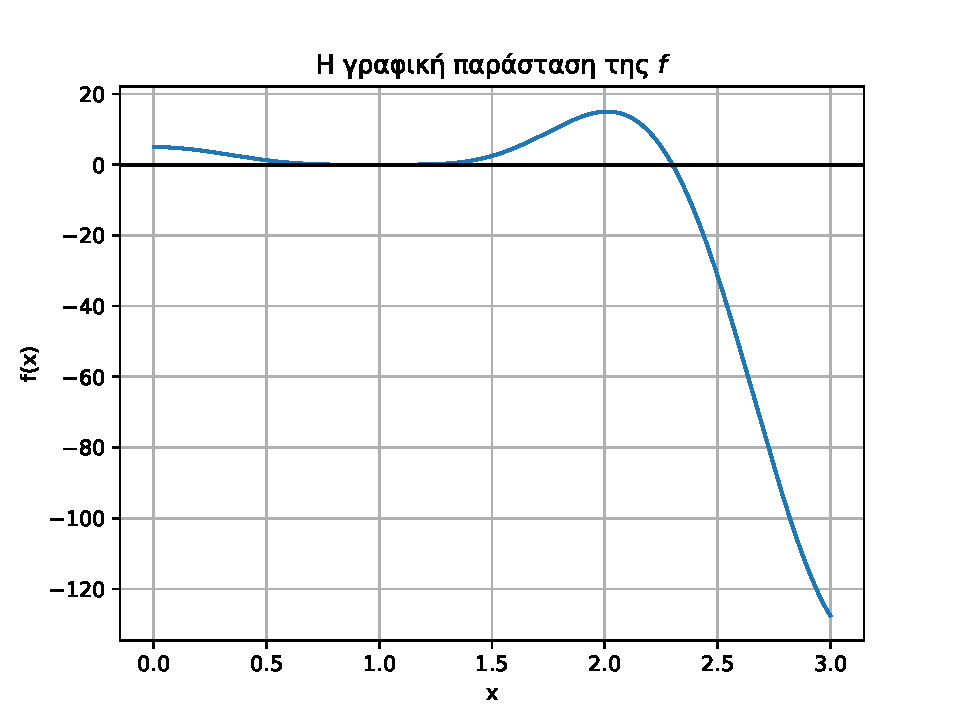
\includegraphics[width=\linewidth]{Exercise2/f_figure.pdf}\\

Μπορούμε να παρατηρήσουμε ρίζες στα διαστήματα $[0.5, 1.5]$ και $[2.0, 2.5]$. Αν μελετήσουμε την συνάρτηση πιο αναλυτικά θα παρατηρήσουμε ότι στο διάστημα $[0.5, 1.5]$ δεν έχει μία ρίζα αλλά δύο. Για αυτό τον λόγο είναι χρήσιμο να κάνουμε την γραφική παράσταση της συνάρτησης στο διάστημα $[0.8, 1.2]$ όπου οι δύο αυτές ρίζες φαίνονται πιο ξεκάθαρα:\\

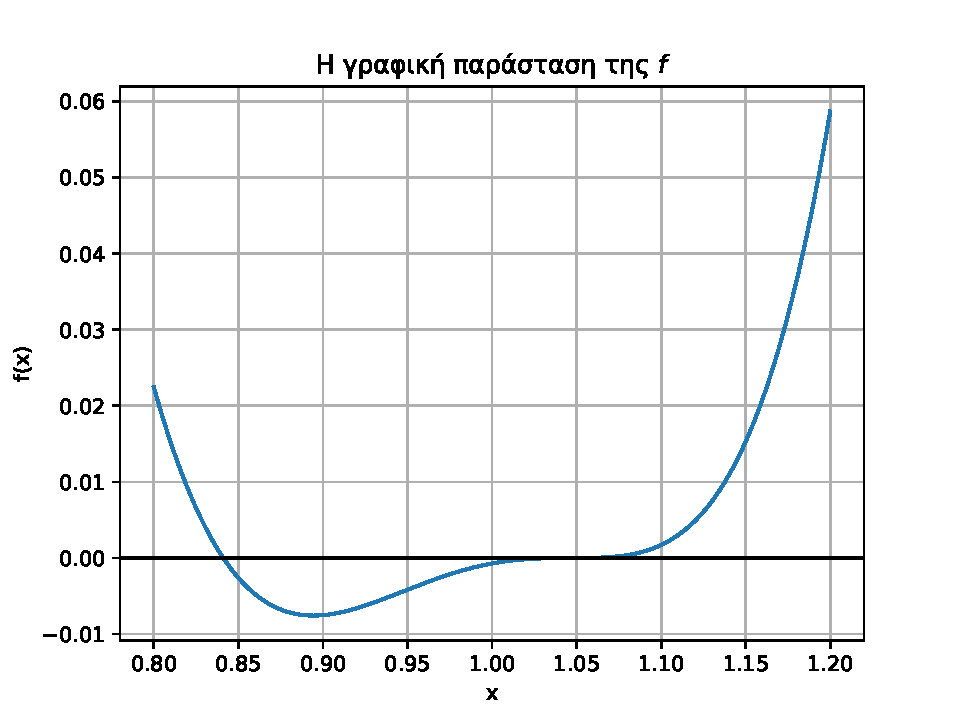
\includegraphics[width=\linewidth]{Exercise2/f_figure_b.pdf}\\

Οπότε έχουμε μία αρχική εκτίμηση της τοποθεσίας των ριζών με την οποία μπορούμε να τροφοδοτήσουμε τους παραπάνω αλγορίθμους για την εύρεση τους.\\

Η εύρεση των ριζών με κάθε έναν απο τους παραπάνω αλγορίθμους γίνεται προγραμματιστικά (σε γλώσσα {\lt python}) στο αρχείο {\lt d\textunderscore 1\textunderscore find\textunderscore f\textunderscore roots.py} το οποίο φαίνεται παρακάτω:

\lt
\lstinputlisting[language=Python]{d_1_find_f_roots.py}
\gt

Στον παραπάνω κώδικα, ορίζω εκ νέου τις συναρτήσεις που υλοποιούν τις τροποιημένες μεθόδους.

Στην συνέχεια ορίζω τις συναρτήσεις {\lt f, f\textunderscore derivative, f\textunderscore second\textunderscore derivative} που υλοποιούν την συνάρτηση $f$ και την πρώτη και δεύτερη παράγωγο της αντίστοιχα.
Ακολούθως, για κάθε ρίζα καλώ την συνάρτηση κάθε μεθόδου (με αντίστοιχες παραμέτρους) και αποθηκεύω τα αποτελέσματα στις μεταβλητές {\lt root, loops\textunderscore counter} που αποθηκεύουν την τελική εκτίμηση της ρίζας και τον αριθμό των επαναλήψεων αντίστοιχα. Μετά, χρησιμοποιώντας αυτές τις μεταβλητές τυπώνω τα αποτελέσματα.\\

Για την τροποποιημένη μέθοδο {\lt Newton-Raphson} χρησιμοποιώ ως αρχικές εκτιμήσεις ριζών τα σημεία: 0.8, 1.0 και 2.3.\\
Για την τροποιημένη μέθοδο διχοτόμησης χρησιμοποιώ ως αρχικά διαστήματα τα: $[0.8, 1.0]$, $[1.0, 1.2]$ και $[2.2, 2.4]$.\\
Για την τροποιημένη μέθοδο τέμνουσας χρησιμοποιώ ως αρχικές 3αδες σημείων ({\lt $x_n, x_{n+1}, x_{n+2}$}) τα: (0.8, 0.85, 0.9), (1.0, 1.1, 1.2) και (2.0, 2.25, 2.5).\\

Άν εκτελέσουμε τον κώδικα θα τυπωθεί:\\
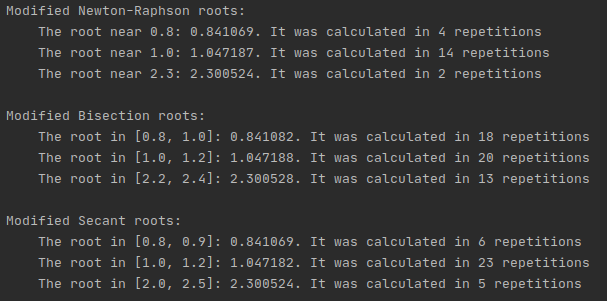
\includegraphics[width=\linewidth]{Exercise2/run_1.png}\\
Μπορούμε να δούμε ότι οι μέθοδοι συγκλίνουν για όλες τις επιλεγμένες αρχικές προσεγγίσεις και:
\begin{itemize}
    \item Η τροποποιημένη μέθοδος {\lt Newton-Raphson} δίνει ως αποτέλεσμα τις ρίζες: 0.841069 (σε 4 επαναλήψεις), 1.047187 (σε 14 επαναλήψεις) και 2.300524 (σε 2 επαναλήψεις).
    \item Η τροποιημένη μέθοδος διχοτόμησης δίνει ως αποτέλεσμα τις ρίζες: 0.841082 (σε 18 επαναλήψεις), 1.047188 (σε 20 επαναλήψεις) και 2.300528 (σε 13 επαναλήψεις) (τα αποτελέσματα σε επόμενη εκτέλεση του ίδιου αρχείου αναμένεται να διαφέρουν λόγω της τυχαιότητας που λαμβάνει μέρος στον υπολογισμό της ρίζας).
    \item Η τροποιημένη μέθοδος τέμνουσας δίνει ως αποτέλεσμα τις ρίζες: 0.841069 (σε 6 επαναλήψεις), 1.047182 (σε 23 επαναλήψεις) και 2.300524 (σε 5 επαναλήψεις).
\end{itemize}

\section{Ερώτημα (2): Έλεγχος σύγκλισης τροποιημένης μεθόδου διχοτόμησης}
Ζητείται να γίνει εκτέλεση του αλγορίθμου τροποιημένης μεθόδου διχοτόμησης και να διαπιστωθεί το αν συγκλίνει πάντα σε ίδιο αριθμό επαναλήψεων.\\

Προγραμματιστικά αυτο γίνεται (σε γλώσσα {\lt python}) στο αρχείο\\ {\lt d\textunderscore 2\textunderscore modified\textunderscore bisection\textunderscore convergence.py} το οποίο φαίνεται παρακάτω:\\
\lt
\lstinputlisting[language=Python]{d_2_modified_bisection_convergence.py}
\gt

Στον παραπάνω κώδικα, ορίζω εκ νέου την συνάρτηση που υλοποιεί την τροποποιημένη μέθοδο διχοτόμησης και στην συνέχεια ορίζω την συνάρτηση {\lt f} που υλοποιεί την $f$ της οποίας τις ρίζες ζητήθηκε να βρώ στο ερώτημα 1 (\lt $f(x) = 94cos^3x - 24cosx + 177sin^2x - 108sin^4x - 72cos^3xsin^2x -65$ \gt).\\
Στην συνέχεια εκτελώ για κάθε ρίζα την τροποποιημένη μέθοδο διχοτόμησης 10 φορές (με τα ίδια ορίσματα με τα οποία κλήθηκε στο ερώτημα 1) και τυπώνω τα αποτελέσματα.\\

Άν εκτελέσουμε τον κώδικα θα τυπωθεί:\\
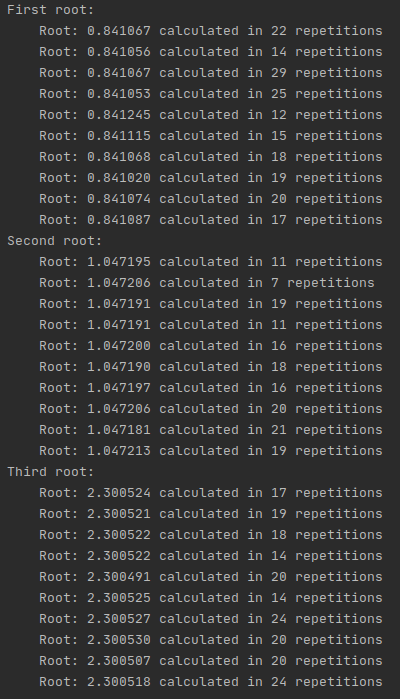
\includegraphics[width=200pt]{Exercise2/run_2.png}\\

Σύμφωνα με το παραπάνω διαπιστώνουμε ότι δεν συγκλίνει σε ίδιο σταθερό αριθμό επαναλήψεων.

\section{Ερώτημα (3): Σύκριση ταχύτητας σύκλισης τροποποιημένων μεθόδων σε σχέση με τις κλασσικές}
Ζητείται να γίνει συγκριση ως προς την ταχύτητα σύγκλισης των τροποιημένων μεθόδων σε
σχέση με τις κλασικές με πειραματικό τρόπο.\\

Προγραμματιστικά αυτο γίνεται (σε γλώσσα {\lt python}) στο αρχείο {\lt d\textunderscore 3\textunderscore compare\textunderscore with\textunderscore classic.py} το οποίο φαίνεται παρακάτω:\\
\lt
\lstinputlisting[language=Python]{d_3_compare_with_classic.py}
\gt

Στον παραπάνω κώδικα, αρχικά ορίζονται εκ νέου οι  συναρτήσεις που υλοποιούν τις τροποποιημένες μεθόδους.\\
Στην συνέχεια, ορίζω τις μεθόδους {\lt classic\textunderscore bisection}, {\lt classic\textunderscore newton\textunderscore raphson} και {\lt classic\textunderscore secant} που υλοποιούν τις κλασσικές μεθόδους διχοτόμησης, {\lt Newton-Raphson} και τέμνουσας αντίστοιχα. Ο κώδικας τον οποίον η κάθε μία υλοποιεί είναι πανομοιότυπος με εκείνον της αντίστοιχης μεθόδου του αντίστοιχου ερωτήματος της άσκησης 1 και για αυτό παραλείπεται η ανάλυση του.\\
Στην συνέχεια ορίζω τις συναρτήσεις {\lt f, f\textunderscore derivative, f\textunderscore second\textunderscore derivative} που υλοποιούν την συνάρτηση $f$ και την πρώτη και δεύτερη παράγωγο της αντίστοιχα. Ως $f$ ορίζεται η συνάρτηση της οποίας οι ρίζες ζητήθηκε να βρεθούν στο ερώτημα 1 (\lt $f(x) = 94cos^3x - 24cosx + 177sin^2x - 108sin^4x - 72cos^3xsin^2x -65$ \gt)\\

Τέλος, για κάθε μέθοδο (κλασσική και έπειτα τροποποιημένη) βρίσκω κάθε ρίζα με τις κατάλληλες παραμέτρους που είναι ίδιες με αυτές που χρησιμοποιήθηκαν για εύρεση των ριζών της $f$ στο ερώτημα 1 και τυπώνω τα αποτελέσματα κάθε εκτέλεσης.\\

Άν εκτελέσουμε το αρχείο θα εμφανιστεί:\\
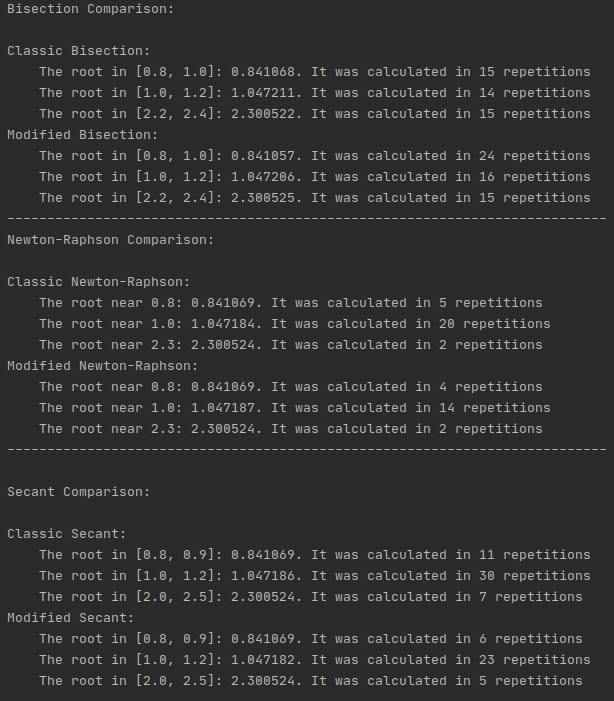
\includegraphics[width=350pt]{Exercise2/run_3.png}\\


\par
Για την μέθοδο της διχοτόμησης:
\begin{itemize}
    \item Για την ρίζα στο $[0.8, 1.0]$ η κλασσική μέθοδος συγκλίνει $24 - 15 = 9$ επαναλήψεις πιο γρήγορα σε σχέση με την τροποποιημένη μέθοδο.
    \item Για την ρίζα στο $[1.0, 1.2]$ η κλασσική μέθοδος συγκλίνει $16 - 14 = 2$ επαναλήψεις πιο γρήγορα σε σχέση με την τροποποιημένη μέθοδο.
    \item Για την ρίζα στο $[2.2, 2.4]$ η κλασσική μέθοδος συγκλίνει με τον ίδιο αριθμό επαναλήψεων σε σχέση με την τροποποιημένη μέθοδο.
\end{itemize}
Επομένως, απο τα παραπάνω διαπιστώνουμε ότι για την μέθοδο της διχοτόμησης η κλασσική μέθοδος είναι, εν γένει, πιο γρήγορη απο την τροποποιημένη.\\

\par
Για την μέθοδο {\lt Newton-Raphson}:
\begin{itemize}
    \item Για την ρίζα κοντά στο 0.8 η τροποποιημένη μέθοδος συγκλίνει $5 - 4 = 1$ επανάληψη πιο γρήγορα σε σχέση με την κλασσική μέθοδο.
    \item Για την ρίζα κοντά στο 1.0 η τροποποιημένη μέθοδος συγκλίνει $20 - 14 = 6$ επαναλήψεις πιο γρήγορα σε σχέση με την κλασσική μέθοδο.
    \item Για την ρίζα κοντά στο 2.3 η τροποποιημένη μέθοδος συγκλίνει με τον ίδιο αριθμό επαναλήψεων με την κλασσική μέθοδο.
\end{itemize}
Επομένως, απο τα παραπάνω διαπιστώνουμε ότι για την μέθοδο {\lt Newton-Raphson} η τροποποιημένη μέθοδος είναι, εν γένει, πιο γρήγορη απο την κλασσική.\\


\par
Για την μέθοδο της τέμνουσας:
\begin{itemize}
    \item Για την ρίζα στο $[0.8, 0.9]$ η τροποποιημένη μέθοδος συγκλίνει $11 - 6 = 5$ επαναλήψεις πιο γρήγορα σε σχέση με την κλασσική μέθοδο.
    \item Για την ρίζα στο $[1.0, 1.2]$ η τροποποιημένη μέθοδος συγκλίνει $30 - 23 = 7$ επαναλήψεις πιο γρήγορα σε σχέση με την κλασσική μέθοδο.
    \item Για την ρίζα στο $[2.2, 2.5]$ η τροποποιημένη μέθοδος συγκλίνει $7 - 5 = 2$ επαναλήψεις πιο γρήγορα σε σχέση με την κλασσική μέθοδο.
\end{itemize}
Επομένως, απο τα παραπάνω διαπιστώνουμε ότι για την μέθοδο της τέμνουσας η τροποποιημένη μέθοδος είναι πιο γρήγορη απο την κλασσική.



\end{document}
